%--------------------------------------------------------------------------------------------------
% OBSERVACAO:
% 
% -> Arquivos que você pode editar:
%    - artigo.tex
%    - artigo_bibliografia.bib
%
% -> Arquivo .TeX codificado em UTF8                                                             
% -> Bibliografia em arquivo .bib (arquivo_bibliografia.bib)                                      
% -> Arquivo de imagens em .jpg, .eps ou .pdf
% -> Para compilar o TeX, execute 'compila_TEX.bat' (terminal do windows)
% 
% versão 1.1 - 19/05/2016
% versão 1.0 - 18/08/2015
%--------------------------------------------------------------------------------------------------
\documentclass{classe_cn}                 % Modelo <nao edite o arquivo classe_cn.cls>
\usepackage[brazil]{babel}                % Acentos
\usepackage[utf8]{inputenc}               % Codificação UTF8 (atenção aqui!)
\usepackage{graphicx}                     % Figura
\usepackage{amssymb}                      % Simbolos matematicos
\usepackage{color}                        % Cores
\usepackage{amsfonts}                     % Fontes
\usepackage{amsmath}                      % Fontes
\usepackage[fixlanguage]{babelbib}        % Acentos
\usepackage[normalem]{ulem}               % OK
\usepackage[retainorgcmds]{IEEEtrantools} % Formulas padrão IEEE
\usepackage{omlmathbf}                    % Simbolos Matematicos
\usepackage{epstopdf}                     % Figuras .eps
\usepackage{setspace}                     % Espaçamento flexível
\usepackage{cmap}                         % Mapear caracteres especiais no PDF
\usepackage{textcomp}                     % Funções e outros símbolos matemáticos
\usepackage{verbatim}                     % Pacotes verbatim
\usepackage{wrapfig}
\usepackage{picins}
\startlocaldefs
\endlocaldefs

%--------------------------------------------------------------------------------------------------
% Inicio do Documento
%--------------------------------------------------------------------------------------------------
\begin{document}
\begin{frontmatter}        % Não alterar
\begin{fmbox}              % Não alterar
\dochead{Gerência da Informação} % Não alterar

%--------------------------------------------------------------------------------------------------
% Titulo do seu Trabalho
%   - pequeno bug (nao funciona cedilha)
%   - editar manualmente o cedilha na classe_cn.cls, linha 1015.
%--------------------------------------------------------------------------------------------------
\title{Software Livre para Empresas}

%------------------------------------------------
% Informações sobre o autor #1
% - Antunes Dantas da Silva
%------------------------------------------------
\author[
  addressref = {aff1},                 % Identifica o autor #1
  email      = {antunes.dantas@ccc.ufcg.edu.br} % email para contato
]
{
  \inits{ADdS}      % Letras iniciais do autor #1
  \fnm{Antunes Dantas}  % Nome do autor #1 (first and middle name)
  \snm{da Silva}   % Ultimo nome do autor #1 (last name)
}
%------------------------------------------------
% Informações sobre o autor #2
% - Gabriel Silva Vinha
%------------------------------------------------
\author[
  addressref = {aff1},                      % Identifica o autor
  email      = {gabriel.vinha@ccc.ufcg.edu.br} % email para contato
]
{
  \inits{GSV}       % Letras iniciais do autor #2
  \fnm{Gabriel Silva}  % Nome do autor #2 (first and middle name)
  \snm{Vinha}    % Ultimo nome do autor #2 (last name)
}
%------------------------------------------------
% Informações sobre o autor #3
% - Italo M. de L. Poroca
%------------------------------------------------
\author[
  addressref = {aff1},                       % Identifica o autor
  email      = {italo.poroca@ccc.ufcg.edu.br} % email para contato
]
{
  \inits{IMdLP}      % Letras iniciais do autor #3
  \fnm{Italo M. de Lima} % Nome do autor #3 (first and middle name)
  \snm{Poroca}    % Ultimo nome do autor #3 (last name)
}
%------------------------------------------------
% Informações sobre o autor #4
% - Valter V. M. de Lucena
%------------------------------------------------
\author[
  addressref = {aff1},                 % Identifica o autor
  email      = {valter.lucena@ccc.ufcg.edu.br} % email para contato
]
{
  \inits{VVMdL}     % Letras iniciais do autor #4
  \fnm{Valter V. M.} % Nome do autor #4 (first and middle name)
  \snm{de Lucena}     % Ultimo nome do autor #4 (last name)
}

%------------------------------------------------
% Endereço dos autores
%------------------------------------------------
\address[id=aff1]{
  \orgname{Universidade Federal de Campina Grande,
           Centro de Engenharia Elétrica e Informática,
           Departamento de Sistemas e Computação},
  \street{Rua Aprígio Veloso, 882, Bairro Universitário},
  \postcode{58429-140},
  \city{Campina Grande},
  \cny{Brasil.}
}

\end{fmbox}

%--------------------------------------------------------------------------------------------------
% Resumo do Trabalho
%--------------------------------------------------------------------------------------------------
\begin{abstractbox}
	
\begin{abstract} 
Escrever no máximo $150$ palavras no resumo do trabalho. Exemplo: The objective of this work is to determine if people are interacting in TV video by detecting whether they are looking at each other or not.We determine both the temporal period of the interaction and also spatially localize the relevant people. We make the following four contributions: (\textit{i}) head detection with implicit coarse pose information (front, profile, back); (\textit{ii}) continuous head pose estimation in unconstrained scenarios (TV video) using Gaussian process regression; (\textit{iii}) propose and evaluate several methods for assessing whether and when pairs of people are looking at each other in a video shot; and (\textit{iv}) introduce new ground truth annotation for this task, extending the TV human interactions dataset. The performance of the methods is evaluated on this dataset, which consists of $300$ video clips extracted from TV shows. Despite the variety and difficulty of this video material, our best method obtains an average precision of $87.6\%$ in a fully automatic manner.
\end{abstract}

%--------------------------------------------------------------------------------------------------
% Palavras-chaves: Entre 3 e 6 palavras chaves
%--------------------------------------------------------------------------------------------------
\begin{keyword}
  \kwd{Escreva}
  \kwd{algumas}
  \kwd{palavras-chaves}
  \kwd{aqui!}
\end{keyword}

\end{abstractbox} % Não alterar
\end{frontmatter} % Não alterar

%--------------------------------------------------------------------------------------------------
% Escreva o seu artigo!
%--------------------------------------------------------------------------------------------------

%------------------------------------------------
% Seção 1
%------------------------------------------------
\section{Introdução}

O \textit{software} livre é uma realidade que existe desde os primórdios da computação. Baseando-se na ideia básica de que o código fonte deve ser público, o movimento do \textit{software} livre gerou, e ainda gera, bastante polêmica dentre a comunidade da tecnologia da informação, especialmente quando o assunto tange as grandes corporações que lucram com a venda de \textit{softwares} proprietários. Como movimento, iniciou em 1983 com um americano chamado Richard Stallman, que liderou o desenvolvimento de um sistema operacional baseado totalmente nas ideias do \textit{software} livre.

Para ser considerado livre, um \textit{software} deve seguir determinadas "leis", que definem como ele deve ser publicado. Para facilitar a publicação, foram criadas licenças genéricas que servem para qualquer \textit{software}.

Um dos principais questionamentos quando o assunto é tratado é como empresas podem faturar fabricando código aberto. Como será exposto posteriormente, existem diversos modelos de negócios que podem ser abordados para este fim.

Este artigo seguirá a seguinte estrutura: na seção 2, será mostrada a motivação para este estudo. Na seção 3, o tema \textit{software} livre será abordado de maneira mais detalhada, bem como modalidades que onde este é encontrado. Na seção 4, será realizado um breve estudo sobre as principais licenças de publicação. Finalmente, na seção 5, será tratado como empresas podem fazer o uso de \textit{software} livre: tanto no lado cliente quanto no lado empresas produtoras. A seção 6 fará uma discussão sobre o futuro da distribuição dos \textit{softwares} e como o \textit{software} livre se encaixa nessa realidade futura.


%------------------------------------------------
% Seção 2
%------------------------------------------------
\section{Motivação}

If we assume that sensitive cells follow a deterministic decay $Z_0(t) = xe^{\lambda_0 t}$ and approximate their extinction time as $T_x \approx \frac{1}{\lambda_0} \log x$, then we can heuristically estimate the expected value as:

\begin{eqnarray}
\label{eqexpmuts}
  E [Z_1(vT_x)] &=& \frac{\mu}{r}\log x \int_0^{1} x^{1-u} du \\
  E [Z_1(vT_x)] &=& \frac{\mu}{r}x^{1-{\lambda_1}/{\lambda_0}v}\log  \\
  1 &=& 10
\end{eqnarray}

\begin{equation}
  E [Z_1(vT_x)] = \frac{\mu}{r}\log x \int_0^{1} x^{1-u} du \\
  E [Z_1(vT_x)] = \frac{\mu}{r}x^{1-{\lambda_1}/{\lambda_0}v}\log 
\end{equation}

Thus we observe that this expected value is finite for all $v>0$ (also see \cite{Rosenfeld:1970}).

%------------------------------------------------
% Sub-seção
%------------------------------------------------
\subsection{Exemplo de Sub-Seção}

In this section we examine the growth rate of the mean of $Z_0$, $Z_1$ and $Z_2$. In addition, we examine a common modeling assumption and note the importance of considering the tails of the extinction time $T_x$ in studies of escape dynamics. We will first consider the expected resistant population at $vT_x$ for some $v>0$, (and temporarily assume $\alpha=0$).

\begin{eqnarray}
E [Z_1(vT_x)]= \mu T_x \int_{0}^{\inf} \lambda_1T_x(v-u)du
\end{eqnarray}

If we assume that sensitive cells follow a deterministic decay $Z_0(t)=xe^{\lambda_0 t}$ and approximate their extinction time as $T_x\approx-\frac{1}{\lambda_0}\log x$, then we can heuristically estimate the expected value as.

%------------------------------------------------
% Exemplo de Tabela
%------------------------------------------------
\section{Software Livre}

Table~\ref{tag_tabela_01} shows the average $ \alpha $ and the standard deviation for the CCR \cite{Rosenfeld:1970} obtained by the \textit{GLCM+SOM} method. We can conclude that for the Brodatz dataset~\cite{Domingues:2010} the processing tool based on mean vectors is the best option~\cite{Rosenfeld:1970, Diday:1989}. Considering this result~\cite{Visible:2013}, the mean vector approach is adopted as processing tool of the \textit{GLCM+SOM} method for the next experiments \cite{Fulano:2009}.

testando 123

% Use a ferramenta para criar tabelas: http://www.tablesgenerator.com/
\begin{table}[h!]
\label{tag_tabela_01}
\caption{Sample table title. This is where the description of the table should go.}
  \begin{tabular}{cccc}
  \hline
       & B1   & B2   & B3   \\ \hline
   A1  & 0.1  & 0.2  & 0.3  \\
   A2  & ...  & ..   & .    \\
   A3  & ..   & .    & .    \\ \hline
  \end{tabular}
\end{table}

\subsection{Software as a Product}

aqui vc faz

\subsection{Software as a Service}

olar

\subsection{Componentes da Produção de Software}

acesso ao software

\section{Licenças de Publicação}

tarara

\section{Software Livre Para Empresas}

O uso de \textit{software} livre em ambientes domésticos e comerciais tem crescido bastante nos últimos anos. O governo brasileiro, inclusive, tem investido bastante em soluções livres nos seus computadores. O mercado em geral também está abraçando a ideia e isso tem feito com que cada vez mais empresas surjam com foco no desenvolvimento de aplicaçãoes baseadas em \textit{software} livre.

Para o cliente, há inúmeros benefícios no uso de \textit{software} livre em suas máquinas. Em primeiro lugar: economia. Para o usuário final, isso significa menos um custo. Para empresas, uma enorme economia.

Para facilitar, pode-se imaginar uma empresa imaginária de \textit{call center}: em uma empresa deste tipo, há muitos computadores. A empresa imaginária teria 1000 computadores para uso dos atendentes mais 200 computadores para uso de supervisores e gerentes. No total 1.200 máquinas que precisam de um sistema operacional e, no caso das máquinas dos supervisores e gerentes, suíte de escritório.

Levando em conta que o custo médio da licença de um sistema operacional proprietário é R\$ 200,00, apenas com este recurso, a empresa gastaria R\$ 240.000,00. Com o uso de \textit{software} livre, a empresa economizaria bastante dinheiro ao adotar um sistema operancional de código aberto, como o Debian.

Além do benefício financeiro, \textit{softwares} livres são, geralmente, mais seguros. Isso acontece por que com o código fonte disponível, qualquer programador pode descobrir um \textit{bug} (erro) e submeter uma correção para ele. O Linux, \textit{kernel} de sistema operacional livre mais difundido no mundo é considerado o sistema operacional mais seguro.

Outro benefício é a facilidade na alteração do funcionamento de algum programa. Com o código aberto, um empresário, por exemplo, pode requisitar a alguma empresa que altere o comportamento de um programa, ou acrescente algo, para adequá-lo à sua realidade e aos seus problemas.

Porém, para o lado das fabricantes de \textit{software}, quais as vantagens de fabricar \textit{software} livre?

Muitas pessoas quando ouvem o termo \textit{software} livre o associam à \textit{software} gratuito. Isso não é verdade. \textit{Software} livre não quer dizer \textit{software} gratuito e existem diversas abordagens comerciais que podem ser utilizadas para monetizar programas de código aberto.

Existem inúmeras empresas que lucram com o \textit{software} livre. A Canonical, desenvolvedora da distribuição Linux Ubuntu tem uma receita anual de \$ 65,7 milhões de dólares. Ela se mantém através de doações e acordos comerciais para inserir conteúdo patrocinado dentro dos seus \textit{softwares}.

A Mozilla, empresa responsável pelo popular navegador de internet Firefox tem uma receita de \$ 330 milhões de dólares anuais. O Firefox, mesmo sendo  um \textit{softwares} livre, gera boa parte dessa receita através de acordo com empresas para agregação de serviços (como o Google Search ser o buscador padrão do navegador) e propagandas em algumas seções do navegador, como a aba "Nova Guia".

A Red Hat é, sem dúvida, uma das mais bem sucedidas empresas no ramo do \textit{softwares} livre. Ela atua através do fornecimento de soluções corporativas. Seus principais produtos são armazenamento, sistemas operacionais, consultoria, treinamento e suporte. Ela utiliza várias abordagens de mercado para vender seus serviços e isso tem dado muito certo. Em 2014, sua receita foi de \$ 1,53 bilhões de dólares. Seus serviços são amplamente utilizados e bem aceitos no mercado.

Essas empresas todas trabalham desenvolvendo \textit{software} livre e tem uma receita considerável. Existem inúmeros outros exemplos de sucesso com o \textit{software} livre: Android, Apache, LibreOffice, Swift são exemplos de aplicações de sucesso no mundo do \textit{software} livre. 

Existem inúmeras abordagens de mercado para fatura com \textit{software} livre. Venda de suporte, treinamento, consultoria, propaganda, dentre outros, são alguns exemplos disso. A seguir, será apresentado as três principais abordagens de mercado para o \textit{software} livre.

\subsection{estatisticas de mercado para saap}
oi


\subsection{Software as a service}

aqui vc faz

\subsection{Open Core}



\section{Tendências}

olar


%--------------------------------------------------------------------------------------------------
%--------------------------------------------------------------------------------------------------
% Define o arquivo BIB (bibliografia)
%--------------------------------------------------------------------------------------------------
%--------------------------------------------------------------------------------------------------
\bibliographystyle{bmc-mathphys}   % NAO EDITAR!
\bibliography{artigo_bibliografia} % NAO EDITAR! - Bibliography file (usually '*.bib' )

\vspace{1.0cm}
\parpic{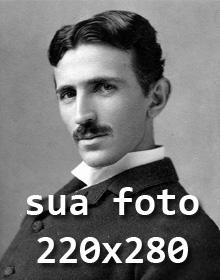
\includegraphics[width=1.5in,clip,keepaspectratio]{tesla.jpg}}
\noindent {\bf Fulano de Tal} was born in India. She received the B.S. 
degree in computer science from Kurukshetra University, Kurukshetra, 
India and the M.Phil. and Ph.D. degrees from the University of Exeter, 
Exeter, UK in 1999, 2001 and 2004, respectively. Her Ph.D. was in the 
area of machine learning for image analysis in aviation security. Her 
main research interests include image processing, natural scene analysis,
video analysis, and neural networks. She has published more than 30 papers
in the area of machine learning for image analysis in peer reviewed 
journals and conferences. Currently she is a Senior Research Fellow at
Loughborough University leading the project on imaging for road transport
applications.

\parpic{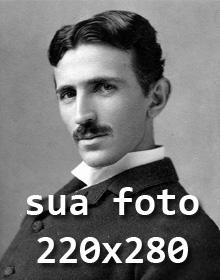
\includegraphics[width=1.5in,clip,keepaspectratio]{tesla.jpg}}
\noindent {\bf Fulano de Tal} was born in India. She received the B.S. 
degree in computer science from Kurukshetra University, Kurukshetra, 
India and the M.Phil. and Ph.D. degrees from the University of Exeter, 
Exeter, UK in 1999, 2001 and 2004, respectively. Her Ph.D. was in the 
area of machine learning for image analysis in aviation security. Her 
main research interests include image processing, natural scene analysis,
video analysis, and neural networks. She has published more than 30 papers
in the area of machine learning for image analysis in peer reviewed 
journals and conferences. Currently she is a Senior Research Fellow at
Loughborough University leading the project on imaging for road transport
applications.   


%\end{tabular}
%\end{table}

%--------------------------------------------------------------------------------------------------
% FIM DO ARTIGO
%--------------------------------------------------------------------------------------------------
\end{document}
